\documentclass{wsdcr}
\usepackage[backend=bibtex]{biblatex}

\addbibresource{rapport.bib}

\title{Étude du model Lotka-Volterra}
\author{Robin Botrel, Axel Carpentier}
\affil{\textit{Université Paul Sabatier}\\
\textit{Toulouse, France}}
\date{28 Decembre, 2022}

\begin{document}

\maketitle
\tableofcontents
\section{Introduction}

\lettrine{C}{ette} étude des équations de prédation de Lotka-Volterra s'effectue dans le cadre d'une unité d'enseignement ouverte de la licence de mathématique de l'université Paul Sabatier. Nous allons partir d'un exercice vu en cours d'équations différentielles ordinaires (EDO), pour ensuite s'éloigner des frontières de ce cours et voir ce que peut offrir la discipline.


\subsection{Le model classique proie prédateur}

Les équations de Lotka-Volterra qualifient un système d'équations différentielles non linéaires, historiquement développées au début du 20ème siècle pour modéliser les interactions entre espèces et plus particulièrement entre 2 espèces : une proie et un prédateur, elles sont un exemple classique d'EDO. Le système est décrit équation \ref{eq:lotka-volterra}. \cite{lotka1920}
\begin{equation}
\left\{
{\begin{array}{ccc}{\dfrac {\mathrm {d} x(t)}{\mathrm {d} t}}&=&x(t)\ {\Big (}\alpha -\beta y(t){\Big )}\\{\dfrac {\mathrm {d} y(t)}{\mathrm {d} t}}&=&y(t)\ {\Big (}\delta x(t)-\gamma {\Big )}\end{array}}
\right.
\label{eq:lotka-volterra}
\end{equation}

%% the title 
\begin{center}
    \fontsize{10}{12}\fontfamily{phv}\fontshape{sc}\selectfont
    \textbf{Un peu d'histoire des mathématiques}
\end{center}

Dans sa publication de 1920 (c'est la première appartion sous cette forme de l'équation \ref{eq:lotka-volterra}), Lokta introduit son model comme un simple cas particulier d'interaction entre deux espèces : La source de nourriture de l'espèce 1 (notée $S_1$) est en excès et peut donc être considérée constante sur la période donnée. l'espèce $S_2$ se nourrit exclusivement de $S_1$.
Il introduit son raisonnement, $X_i$ est la masse de l'espèce $S_i$ :
\begin{equation}
\begin{aligned}
&\begin{bmatrix}
\text{Variation de }X_1 \\ \text{par unité de temps}
\end{bmatrix}
=
\begin{bmatrix}
X_1\text{ engendré}\\ \text{par unité de temps}
\end{bmatrix} \\
&- 
\begin{bmatrix}
X_1\text{ détruit par }X_2\\ \text{par unité de temps}
\end{bmatrix}
-
\begin{bmatrix}
\text{autre perte de }X_1\\ \text{par unité de temps}
\end{bmatrix} \\
&\begin{bmatrix}
\text{Variation de }X_2 \\ \text{par unité de temps}
\end{bmatrix}
=
\begin{bmatrix}
X_2\text{ engendré par l'ingestion de }X_1\\ \text{par unité de temps}
\end{bmatrix} \\
&-
\begin{bmatrix}
\text{autre perte de }X_2\\ \text{par unité de temps}
\end{bmatrix} 
\end{aligned}
\end{equation}
Pour translater ce raisonnement en un système d'EDO, il va faire de nouvelles assomptions, citons Lotka :
\begin{quotation}
Pour de petits changements, le taux de formation de nouvelle matière d'une espèce donnée d'organisme dans des conditions déterminées est proportionnel à la masse existante de cette espèce. En d'autres termes, la croissance de la matière vivante est un processus typiquement "autocatakinetic". […]. La proportionnalité ne s'applique pas aux grandes variations de X1, X2, ce qui est dûment pris en compte dans la mesure où $A_1'$, est une fonction de $X_1$, $X_2$. […]. De même, la masse de $S_1$ détruite par $S_2$ qui s'en nourrit sera, pour de petites variations, proportionnelle à $X_2$ et aussi à $X_1$. Ce terme a donc été défini sous la forme $B_1X_1X_2$. Ici encore, les écarts de proportionnalité sont pris en charge par les variations de $B_1$ avec $X_1$ et $X_2$, variables dont $B_1$ est une fonction.
\end{quotation}
\begin{equation}
\begin{aligned}
{\dfrac {\mathrm {d} X_1(t)}{\mathrm {d} t}}&=A_1^\prime X_1-B_1X_1X_2-A_1^{\prime \prime}X_1\\
{\dfrac {\mathrm {d} X_2(t)}{\mathrm {d} t}}&=A_2X_1X_2-B_2X_2
\end{aligned}
\end{equation}
Il construit sa translation vers un système d'EDO sur l'idée de proportionnalité mais tout en traitant cette proportionnalité comme des fonctions du temps. Durant toute la publication il n'envisage pas d'en faire des constantes. C'est Volterra qui en 1926 dans des lettres à Umberto D'Ancona, décrit la même équation mais tel que AB soit fixes, c'est l'équation que l'on a décrite eq.\ref{eq:lotka-volterra}. Volterra ne semble pas connaître les résultats précédents de Lotka. \cite{volterra1926} \\
Prenons le temps d'étudier certaines propriétés de ce système non linéaire, ces propriétés seront valables pour les généralisations présentés dans la prochaine section. Premièrement, L'EDO est sous formes résolues. Posons $F(t,x,y)=(F_1,F_2)=(x(\alpha -\beta y),y(\delta x-\gamma ))$, Les fonctions $F_1(x,y)$ et $F_2(x,y)$ sont des polynômes à plusieurs indéterminées, il en découle la propriété de régularité $\mathcal{C}^\infty$. Les solutions de l'EDO étant $\mathcal{C}^1$ leur régularité est transmise à la fonction $F(t,x,y)$ en t, la variable n'intervennant pas explicitement. Les solutions sont alors $\mathcal{C}^2$ car elles sont l'intégrale d'une fonction $\mathcal{C}^1$ : $(x,y)(t)-(x,y)(0)=\int_0^t F(s,x,y)ds$, en continuant ce raisonnement on en déduit que les solutions sont $\mathcal{C}^\infty$. \\
On peut alors, dans le cas d'un problème de Cauchy, affirmer l'unicité et l'existence de la solution, F(t,x,y) étant infiniment dérivable, cela implique sa continuité en $t$ ainsi que d'être localement lipschitzienne en (x,y). Pour rappel un problème de Cauchy consiste à se donner une EDO et un vecteur de conditions initiales, ici de taille 2 (EDO de degré 1 et de dimension 2). Les conditions initiales seront majoritairements étudiées dans le quartier positif du plan $(\mathbb{R}^+)^2$) pour des raisons historiques d'utilisation de ce modèle en écology des populations. \\
Nous étudirons dans les détails les points fixes et les propriétés d'un tel système dans la section \ref{sec:lv2}. En ouverture nous pouvons cependant simuler quelques trajectoires de L'EDO définie eq.\ref{eq:lotka-volterra}.

\subsection{Généralisation}
Comme de nombreux modèles, les équations de Lokta-Volterra ont de nombreuses limitations. Les biologistes et écologistes ont  proposés des améliorations, dans un premier temps en ajoutant un modèle logistique pour limiter la croissance exponentielle des populations, limités non plus par le prédateur ou la proie mais par un environnement à ressources finies. Ce nouveaux modèles présenté equation \ref{eq:clv}, se nomme le modèle compétitif (de Lokta-Volterra).
\begin{equation}
\left\{
{\begin{array}{ccc}{\dfrac {\mathrm {d} x(t)}{\mathrm {d} t}}&=&x(t)\ {\Big (}a -b y(t)-c x(t){\Big )}\\{\dfrac {\mathrm {d} y(t)}{\mathrm {d} t}}&=&y(t)\ {\Big (}d x(t)-e -f y(t) {\Big )}\end{array}}
\right.
\label{eq:clv}
\end{equation}
Dans un même temps, les interactions furent extendues à N espèces, l'EDO se décrit vectoriellement et ses paramètres sont concentrés dans un vecteur définissant l'évolution de la population sans interaction et d'une matrice décrivant les interactions entre espèces et avec l'environnement (modèlisé par la diagonale de la matrice). C'est le modèle généralisé de Lotka-Volterra décrit eq.\ref{eq:glv}. \\
Soit une espèce i et une espèce j, si les coéficients $A_{i,j}$ et $A_{j,i}$ sont de signe négatif, l'interprétation communément admise est une compétition direct deux ces deux espèces, par exemple pour une même ressource. Si les signes sont distincts c'est une interaction proie-prédateur, finalement si les deux signes sont positifs il peut s'agir d'entraide mais le modèle possède des limitations dans ce cas, principalement car cela reconduit à des comportements de croissance exponentielle.
\begin{equation}
\dfrac {\mathrm {d}}{\mathrm {d} t}X(t)=X(t) {\Big (}R+AX(t){\Big )}
\label{eq:glv}
\end{equation}
Dans la prochaine section nous allons nous arrêter sur le cas à deux espèces du modèle généralisé qui, malgré son faible nombre d'espèces, exhibe des comportements intéressants. Malheureusement, nous n'allons pas étudier ce cas dans toute sa généralité, limité par son nombre de paramètres, au nombre de 6 (pouvant tomber jusqu'à 4 avec des changements de variables).
\section{Le cas 2D}
\label{sec:lv2}
Plusieurs visualisations du système : trajectoire (flow?), Champ vectoriel (def), colorbar norme2 de f(X)…
Quels sont les informations que nous pouvons tirer d'un modèle généralisé de Lotka-Volterra, contrairement à certaines EDO il n'est pas possible ici de trouver une solution analytique. Il est néanmoins possible de déterminer de nombreuses propriétés du système analytiquement, en particulier les points d'équilibres ou fixes du système sont l'ensemble des $(x,y)\in \mathbb{R}^2$ où $F(x,y)=0$. Toute trajectoire avec des conditions initiales hors d'un point fixe ne peut l'atteindre en un temps fini, la fonction constante $(x(t),y(t))=(x,y)$ est solution et est unique comme montré précédement. En dynamique des populations, l'isocline $i$ moins restrictive que les points fixes est l'ensemble des points tel que la composante $F_i$ soit nulle.
\begin{equation}
R={\begin{bmatrix}1\\1\end{bmatrix}}\quad A =-{\begin{bmatrix}1&0\\0&1\end{bmatrix}}
\label{eq:RSs0}
\end{equation}
Appliquons ces outils à un cas très simple, l'équation \ref{eq:glv} muni des paramètres définis eq.\ref{eq:RSs0}. On obtient en fait deux équations logistiques découplées, il n'y a pas d'interactions entre les espèces. Étudions la première isocline, $x(1-x)\overset{!}{=}0$ deux solutions s'offrent à nous $x=0$ et $x=1$, les courbes sont donc des droites verticales d'abscisse 0 et 1. La seconde isoline est similaire, les solutions sont $y=0$ et $y=1$. Sur la première isocline $\dot{x}=0$, le champs vectoriel est donc dirigé selon $y$ et le sens du vecteur dépend de l'ordonnée $\dot{y}=y(1-y)$  strictement positif $\forall 0<y<1$. On décompte 4 points fixes ${(0,0),(0,1),(1,0),(1,1)}$ qui résultent de l'intersection des isoclines. Ces informations sont présentés sur le graphe fig.\ref{fig:dessinlv2s0}.
\begin{figure}[t!]
    \centering
    \includegraphics[width=\linewidth]{fig/dessins0.png}
    \caption{dessin}
    \label{fig:dessinlv2s0}
\end{figure}
Vient ensuite l'outil numérique, très puissant dans l'étude des EDO, il introduit cependant de nombreuses approximations. Dans un premier temps il est intéressant d'afficher le champs vectoriel associé à l'EDO, à chaque point $(x,y)$ du plan on associt un vecteur égal à $F(x,y)$, se sont les dérivées tangentes à la trajectoire, la norme des vecteurs est encodée par la couleur pour faciliter la lisibilité de la figure. On peut aussi tracer des trajectoires par une méthode pas à pas, $(x_{t+dt},y_{t+dt})=dt*F(x_{t},y_{t})+(x_{t},y_{t})$ on répète alors l'opération un grand nombre de fois avec $dt$ un pas de temps suffisament petit, c'est la méthode d'Euler explicite. Dû aux nombreuses limitations de cette méthode nous utilisons l'algorithme de Runge Kutta qui offre une meilleure robustesse à l'erreur.
\begin{figure}[t!]
    \centering
    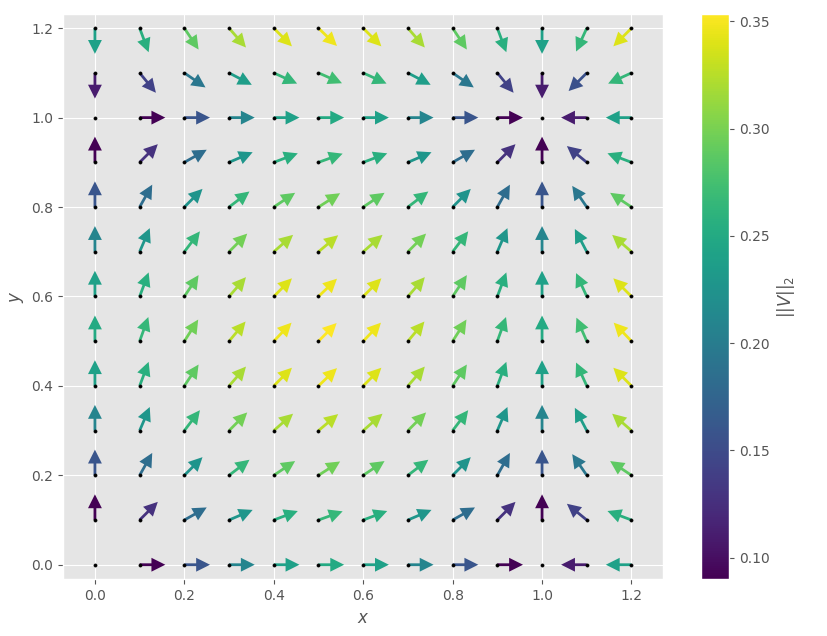
\includegraphics[width=\linewidth]{fig/lv2_vfs0.png}
    \caption{vf}
    \label{fig:vfs0}
\end{figure}
\begin{figure}[t!]
    \centering
    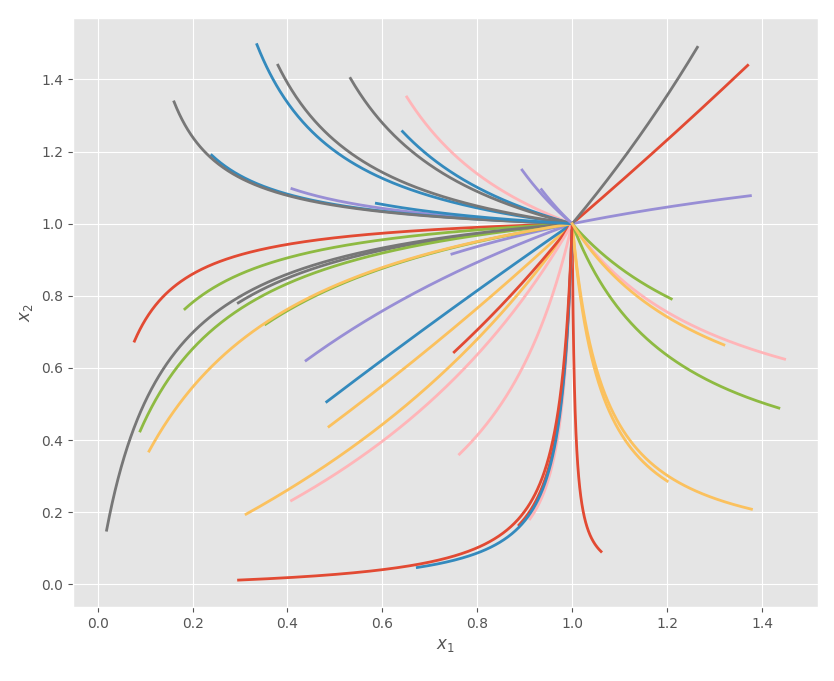
\includegraphics[width=\linewidth]{fig/lv2_ts0.png}
    \caption{traj}
    \label{fig:ts0}
\end{figure}
\begin{equation}
R={\begin{bmatrix}1\\1\end{bmatrix}}\quad A =-{\begin{bmatrix}1&1\\1&1\end{bmatrix}}
\label{eq:RSnInv}
\end{equation}
\begin{figure}[t!]
    \centering
    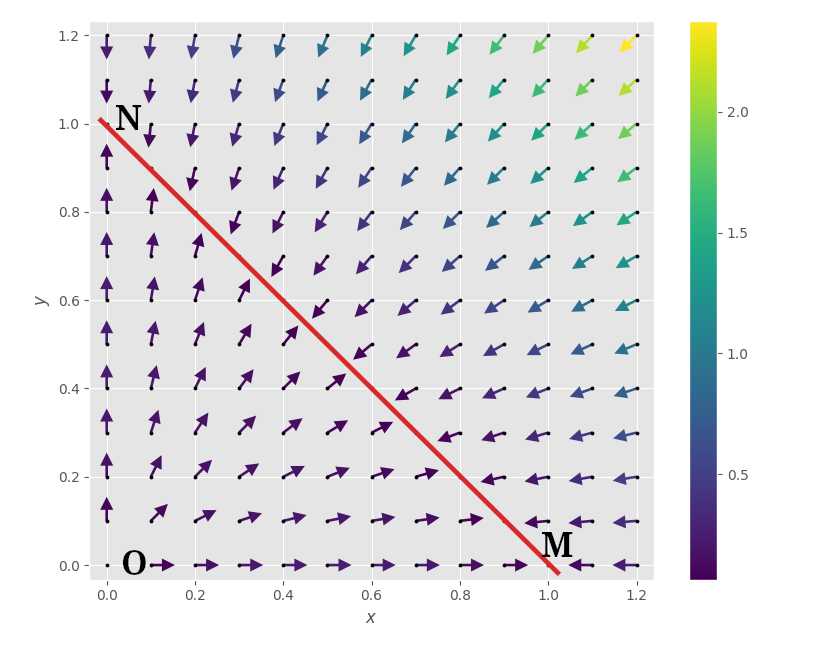
\includegraphics[width=\linewidth]{fig/lv2_vf.png}
    \caption{test}
    \label{fig:vf2}
\end{figure}
\subsection{Une étude des bifurcations}
Le système définit par \ref{eq:RSnInv} possède un comportement étonnant découlant de la non inversibilité de $A$. L'étude des bifurcations a pour object d'étudier l'évolution d'un système dynamique (entres autres ses points d'équilibres) en fonction d'un ou plusieurs paramètres autour d'un changement majeur du système. Il est intéressant dans notre cas d'introduire un paramètre dans $A$ \ref{eq:RSs}, rendant $A(s)$ inversible $\forall s \in \mathds{R}\setminus \{1,-1\}, |A(s)|=1-s^2 \neq 0 $.
\begin{equation}
R={\begin{bmatrix}1\\1\end{bmatrix}}\quad A(s) =-{\begin{bmatrix}1&s\\s&1\end{bmatrix}}
\label{eq:RSs}
\end{equation}
Étudions les points d'équilibres et leurs stabilités de ce système paramétrique \ref{eq:RSs}. 
\begin{equation}
\begin{aligned}
X(R+AX)\overset{!}{=}0 &\land (x_1 = 0 \lor x_2 = 0) \Rightarrow (X=(0,0) \text{(O)} \lor \\ &X=(1,0) \text{(M)}\lor X=(0,1) \text{(N)})\\
X(R+AX)\overset{!}{=}0 &\land (x_1 ´\neq 0 \land x_2 \neq 0 \land s=1) \Rightarrow x_2=1-x_1 \\
X(R+AX)\overset{!}{=}0 &\land (x_1 ´\neq 0 \land x_2 \neq 0 \land s=-1) \Rightarrow X=\varnothing \\
X(R+AX)\overset{!}{=}0 &\land (x_1 ´\neq 0 \land x_2 \neq 0 \land s \neq \pm 1) \Rightarrow X=-A^{-1}R \\ &=\frac{1}{1-s^2}\begin{bmatrix}1&-s\\-s&1\end{bmatrix}\begin{bmatrix}1\\1\end{bmatrix}=\frac{1}{1+s}\begin{bmatrix}1\\1\end{bmatrix} \text{(S)}
\end{aligned}
\label{eq:RSs}
\end{equation}
\begin{equation}
\begin{aligned}
J(f)_X &= \begin{bmatrix}r_1-2x_1-sx_2&-sx_1\\-sx_2&r_2-2x_2-sx_1\end{bmatrix} \\
J(f)_{O} &= \begin{bmatrix}1&0\\0&1\end{bmatrix} \\particular
J(f)_{M} &= \begin{bmatrix}-1&-s\\0&1-s\end{bmatrix} \\
J(f)_{N} &= \begin{bmatrix}1-s&0\\-s&-1\end{bmatrix} \\
J(f)_{S,s\neq \{1,-1\}} &= \frac{1}{1+s}A(s)
\end{aligned}
\end{equation}
À l'aide des Jacobiennes, nous pouvont étudier la stabilité de ces points fixes et donc le comportement local des trajectoires. Soit F un des points fixes. $f$ étant $\mathcal{C}^\infty$ effectuons un développement de taylor à l'ordre 1 en F, sachant que $f(t,F)=0$.
\begin{equation}
f(t,F+H)=J(f)_XH + \mathcal{O}(\|H\|^2) 
\end{equation}
En négligeant les termes d'ordres strictement supérieurs à un, on obtient une nouvelle équation différentielle linéaire, valable localement en F.
\begin{equation}
{\dfrac {\mathrm {d} F+H}{\mathrm {d} t}}={\dfrac {\mathrm {d} H}{\mathrm {d} t}}=J(f)_FH
\end{equation}
Commençons l'analyse des points fixes par le point O dont la matrice jacobienne est invariante par $s$ et est diagonale. On obtient alors le système d'EDO linéaire suivant : 
\begin{equation}
\left\{
{\begin{array}{ccc}{\dfrac {\mathrm {d} h_1(t)}{\mathrm {d} t}}&=&h_1(t)\\{\dfrac {\mathrm {d} h_2(t)}{\mathrm {d} t}}&=&h_2(t)\end{array}}
\right.
\label{eq:JO}
\end{equation}
la solution analytique de l'équation \ref{eq:JO} est $H(t)=\exp(t)Id_2H_0$, autrement dit le point fixe O est expansif, les trajectoires s'éloigne de ce point. \\
$J(f)_{M}$ et $ J(f)_{N}$ sont diagonalisables $\forall s \neq 2$, cette information est déductible de l'étude de $Det(J(f)_{M}-XId_2)=(1-s-X)(1+X)$, le polynôme est scindé à racine simple $\forall s \neq 2$, dans le cas où $s=2$ le polynôme caractéristique $(1+X)^2$ est minimale. Soit $s=2$, résolvons l'EDO par cascade $h_2(t)=C\exp(-t)$ puis $h_1=-2Ct\exp(-t)+D\exp(-t)$. Le comportement obtenu s'observe numériquement en affichant le champ vectoriel autour de M (fig \ref{fig:JM}). \\
\begin{figure}[t!]
    \centering
    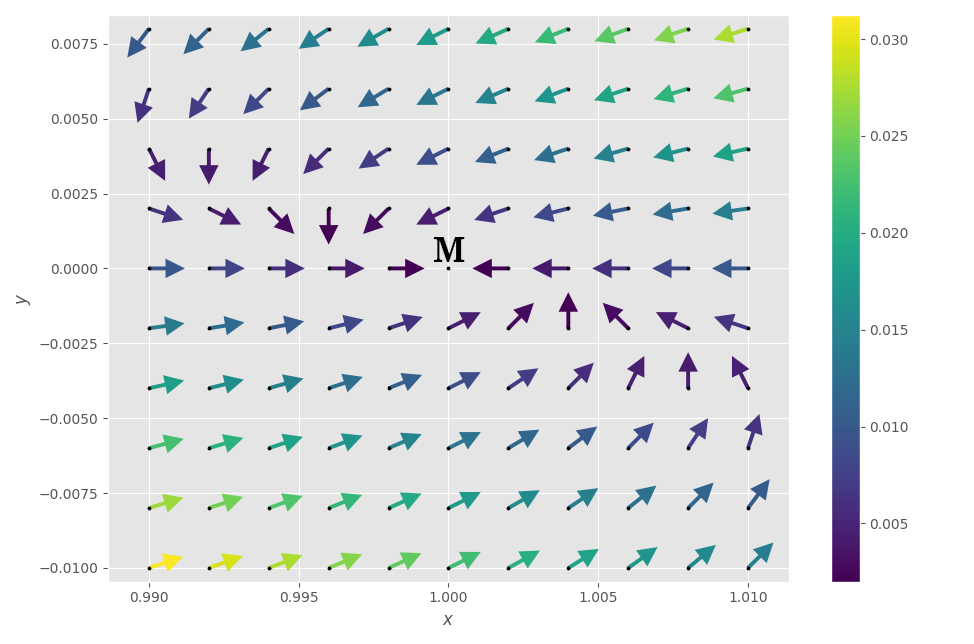
\includegraphics[width=\linewidth]{fig/lv2_vfM.png}
    \caption{test}
    \label{fig:JM}
\end{figure}
Soit $S\neq2 \Rightarrow \exists P \in GL(\mathbb{R}),D \in \mathcal{M}(\mathbb{R}) \text{diagonal}, M = P^{-1}DP$ on a alors ${\dfrac {\mathrm {d} Y}{\mathrm {d} t}}=DY$ avec $Y(t)=PH(t)$ $\lambda_{1,2}$ les valeurs propres, déterminant et trace sont invariants par changement de base et peuvent nous informer sur le signe des valeurs propres en dimension 2.
\begin{itemize}
	\item $s>1 \Rightarrow Det(J(f)_{M})>0 \land Tr(J(f)_{M})<0 \Rightarrow \lambda_i<0$ {\color{red}point stable}
	\item $s=1 \Rightarrow \lambda_1=0 \land \lambda_2=-1$ 
	\item $1>s>0 \Rightarrow Det(J(f)_{M})<0 \land Tr(J(f)_{M})>0 \Rightarrow \lambda_1<0 \land \lambda_2>0$ {\color{red}point selle}
	\item $s=0 \Rightarrow \lambda_1=-1 \land \lambda_2=1$ {\color{red}point selle}
	\item $s<0 \Rightarrow Det(J(f)_{M})<0 \land Tr(J(f)_{M})>0 \Rightarrow \lambda_1<0 \land \lambda_2>0$ {\color{red}point selle}
\end{itemize}
Le cas du point fixe N est similaire au point M. Intéressons nous maintenant au point S. Vérifions que $\forall s \in \mathds{R}\setminus \{1,-1\}$ $J(f)_{S}$ diagonalisable.$Det(J(f)_{S}-XId_2)=\frac{1}{1+s}(\frac{1-s}{1+s}+X)(1+X)$ le polynôme est scindé à racine simple $\forall s \neq 0$ dans le cas où $s=0$ la jacobienne est diagonale. Finalement, $J(f)_{S}$ est diagonalisable $\forall s \in \mathds{R}\setminus \{1,-1\}$. On peut alors étudier le signe du déterminant et de la trace en fonction de $s$ : $Det(J(f)_{S})=\frac{1-s}{1+s}$ et $Tr(J(f)_{S})=\frac{-2}{1+s}$.
\begin{itemize}
	\item $s>1 \Rightarrow Det(J(f)_{S})<0 \land Tr(J(f)_{S})<0 \Rightarrow \lambda_1<0 \land \lambda_2>0$ {\color{red}point selle}
	\item $1>s>-1 \Rightarrow Det(J(f)_{S})>0 \land Tr(J(f)_{S})<0 \Rightarrow \lambda_i<0$ {\color{red}point stable}
	\item $s<-1 \Rightarrow Det(J(f)_{S})<0 \land Tr(J(f)_{S})>0 \Rightarrow \lambda_1<0 \land \lambda_2>0$ {\color{red}point selle}
\end{itemize}
\begin{figure}[t!]
    \centering
    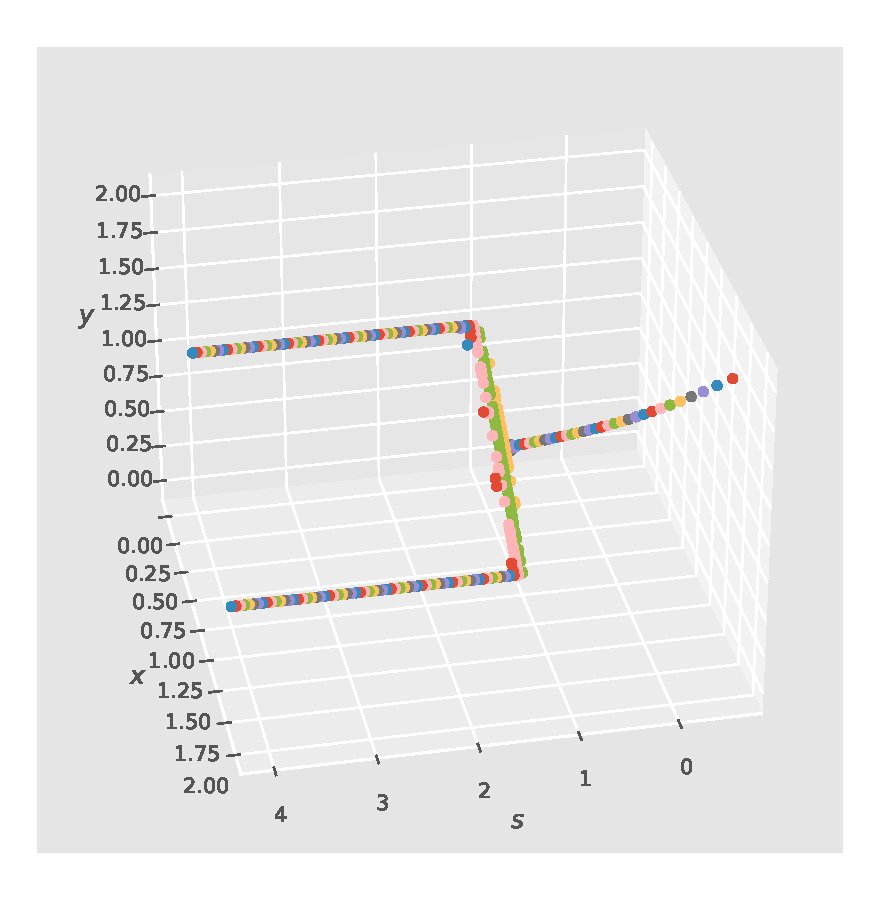
\includegraphics[width=\linewidth]{fig/lv2_bif3Dx10.eps}
    \caption{test}
    \label{fig:bif2}
\end{figure}
On a obtenu toutes les informations nécessaires à la production d'un diagramme des bifurcations de notre système défini eq.\ref{eq:RSs}. Sur la figure.\ref{fig:dessinlv2}, nous avons produit un schema de l'évolution des points fixes en fonction de $s \in [-1,4]$, pour nous limité à un diagramme à deux dimensions nous avons pris en ordonnée la norme 1 $||X||_1$ de la position des points fixes.
\begin{figure}[t!]
    \centering
    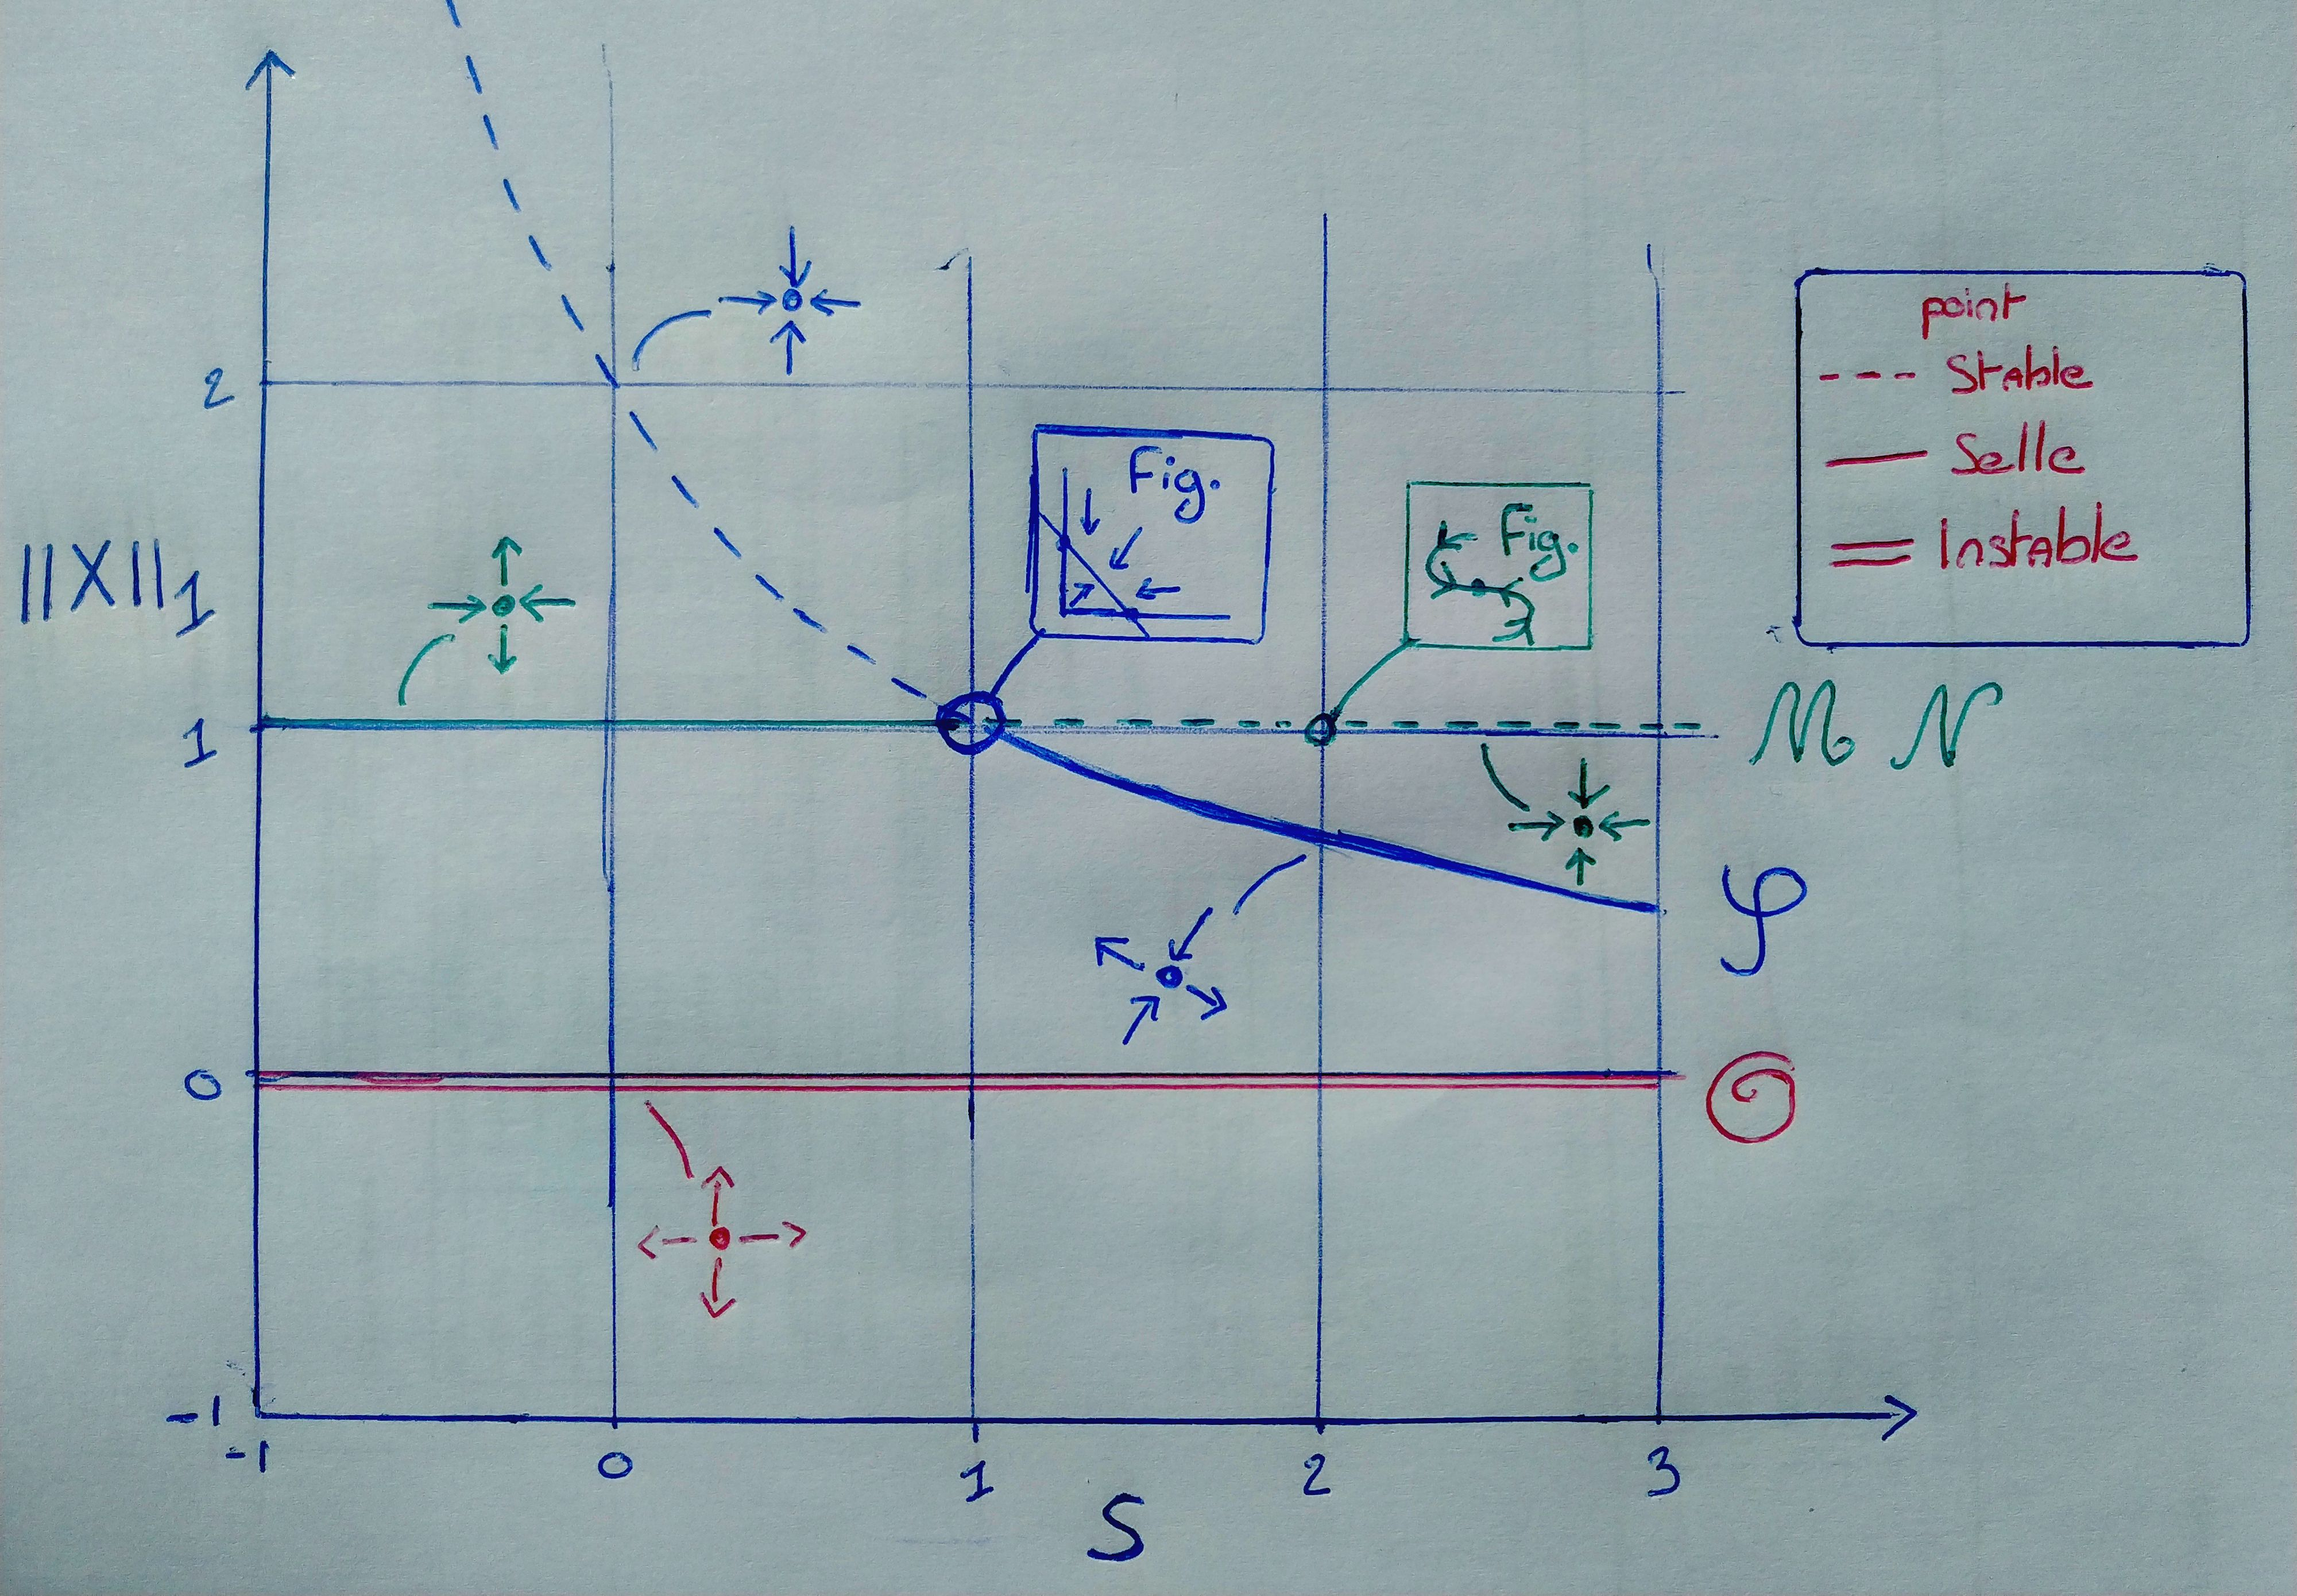
\includegraphics[width=\linewidth]{fig/dessin.png}
    \caption{test}
    \label{fig:dessinlv2}
\end{figure}
Il est intéressant de le comparer à son pendant numérique. La figure \ref{fig:bif2} est le résultat de l'évolution d'une centaine de points tel que $(x_0,y_0) \in [0,1]$ et cela pour chaque valeur de $s \in [-0.5,4]$. On retrouve bien la stabilité de M et N pour $s > 1$ et la stabilité de S pour $(-1<)s<1$. \\
Le comportement que l'on vient d'étudier est intéressant, mais c'est dans les dimensions supérieurs des équations de Lotka-Volterra que se déploient les phénomènes les plus fascinants. Une partie de l'explication de la pauvreté des phénomènes en 2D se trouve dans l'unicité des solutions, les trajectoires ne peuvent se couper, se qui est très limitant en 2D, mais facile à contourner en dimension supérieure. Nous allons donc étudier un système à 4 espèces en interactions directes dans cette prochaine section.
\section{Chaos en 4D}
\subsection{introduction aux attracteurs}
dimension d'apparition
\begin{equation}
R={\begin{bmatrix}1\\0.72\\1.53\\1.27\end{bmatrix}}\quad A =-{\begin{bmatrix}1&1.09&1.52&0\\0&0.72&0.3168&0.9792\\3.5649&0&1.53&0.7191\\1.5367&0.6477&0.4445&1.27\end{bmatrix}}
\end{equation}
\begin{figure}
    \centering
    \subfigure[]{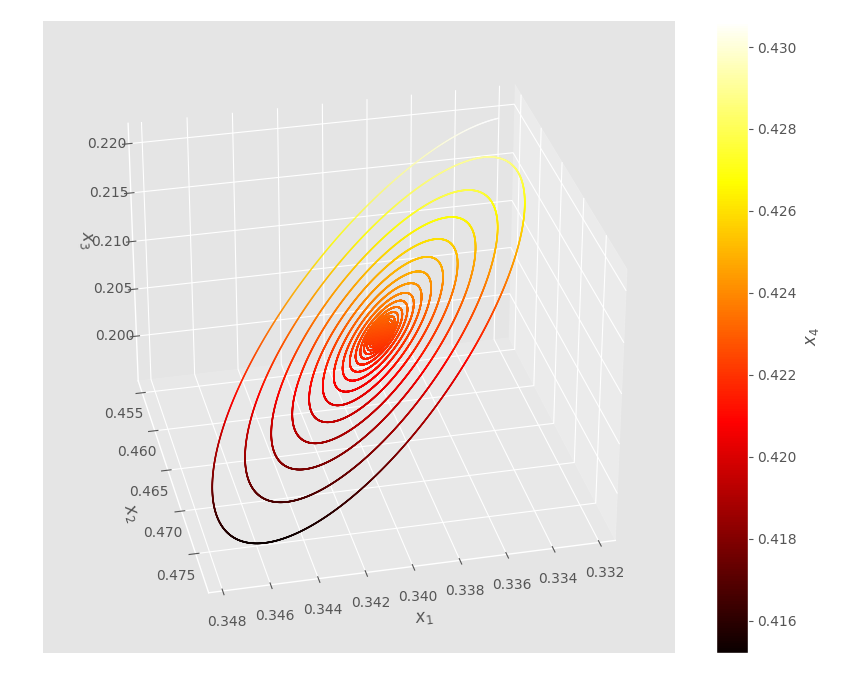
\includegraphics[width=0.3\linewidth]{fig/lv4_ps4.png}} 
    \subfigure[]{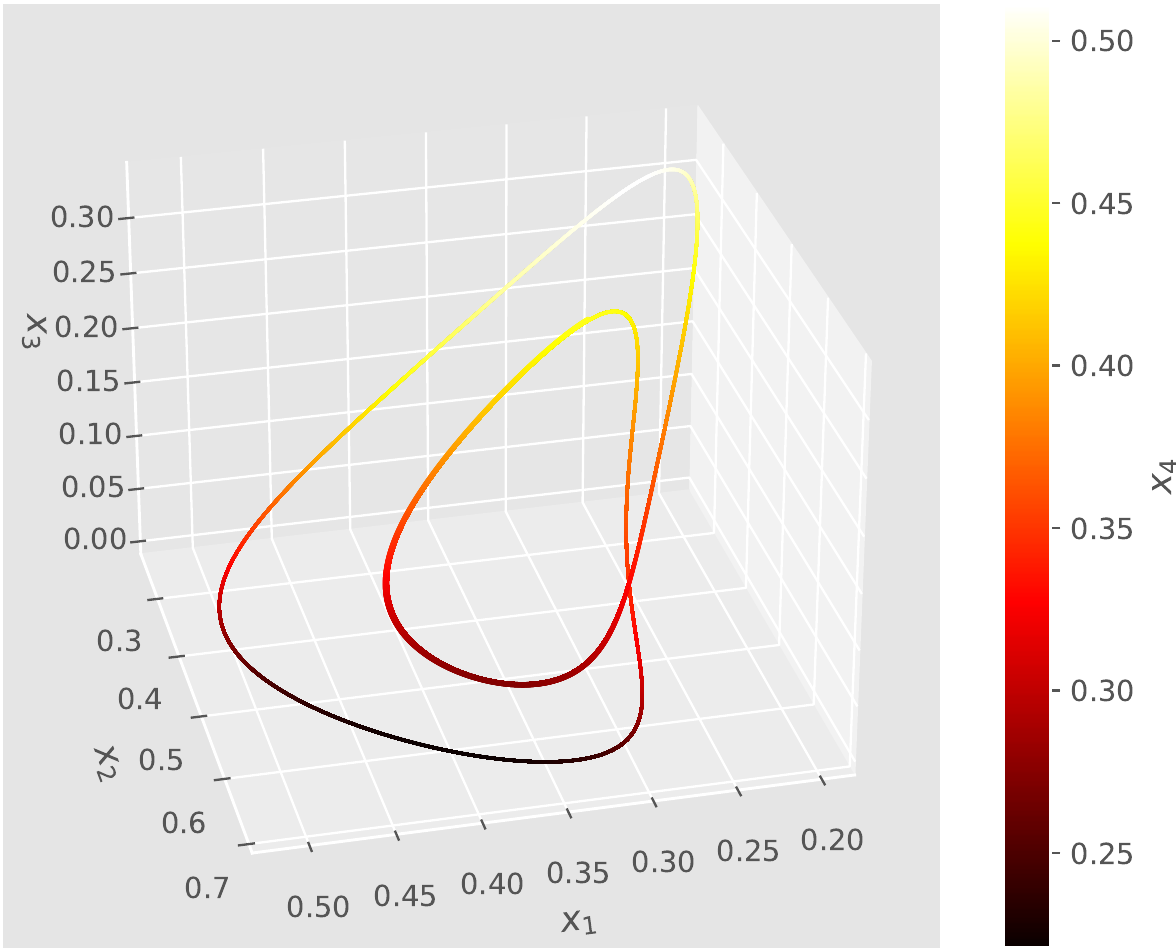
\includegraphics[width=0.3\linewidth]{fig/lv4_cl4.png}} 
    \subfigure[]{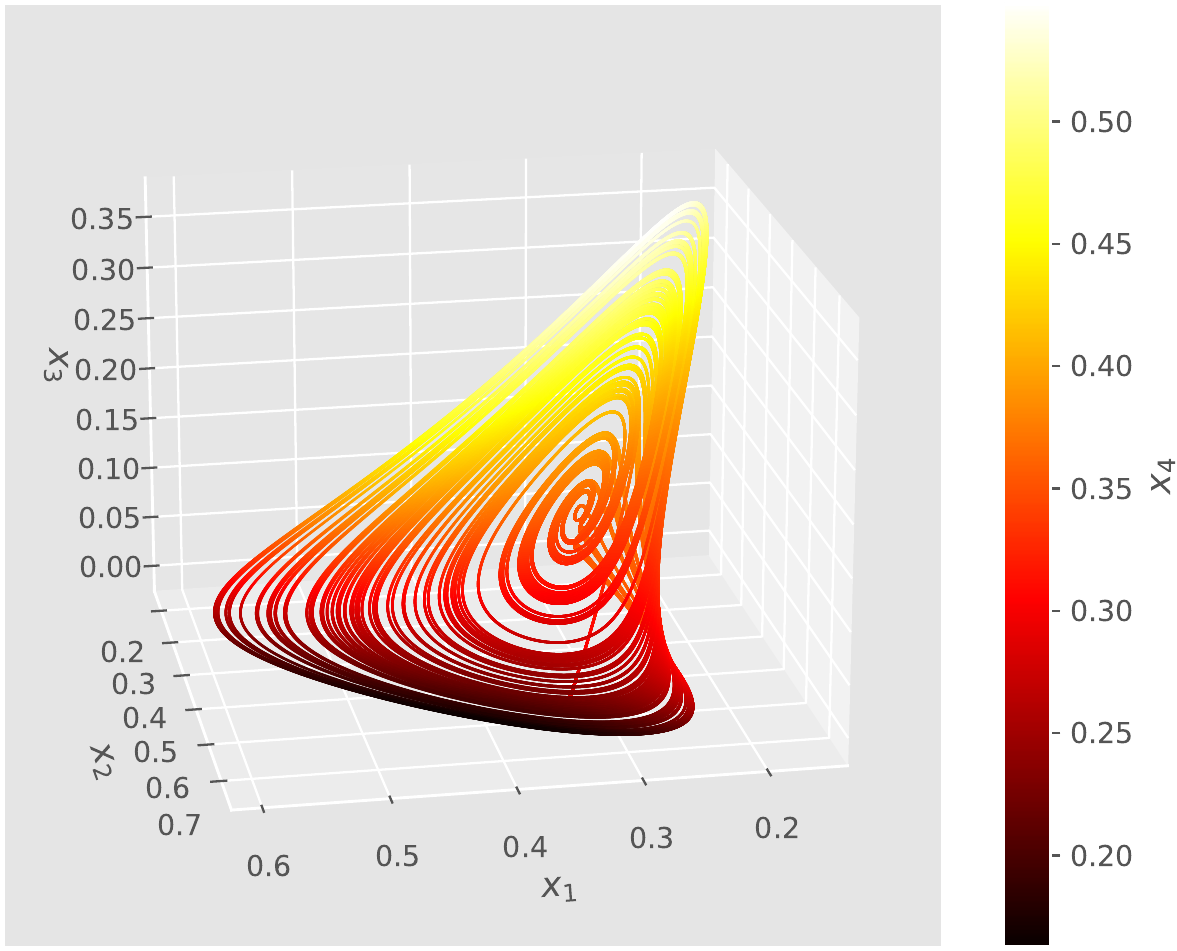
\includegraphics[width=0.3\linewidth]{fig/lv4_ae4.png}}
    \caption{(a) $S=0.8$ (b) $S=0.95$ (c) $S=1$}
    \label{fig:subbif}
\end{figure}
\begin{figure}
    \centering
    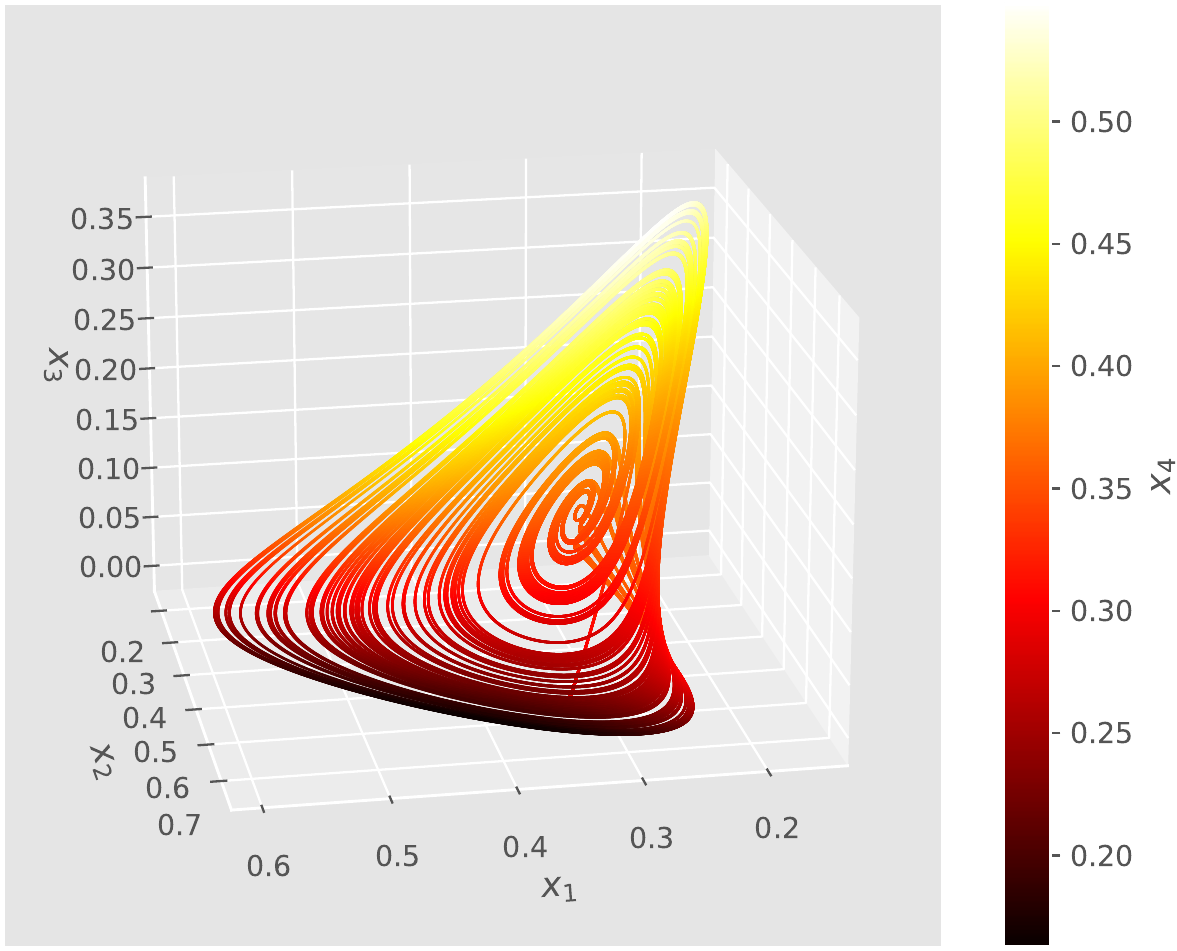
\includegraphics[width=\linewidth]{fig/lv4_ae4.png}
    \caption{attracteur étrange définit par XXX}
    \label{fig:ae4}
\end{figure}
\begin{figure}
    \centering
    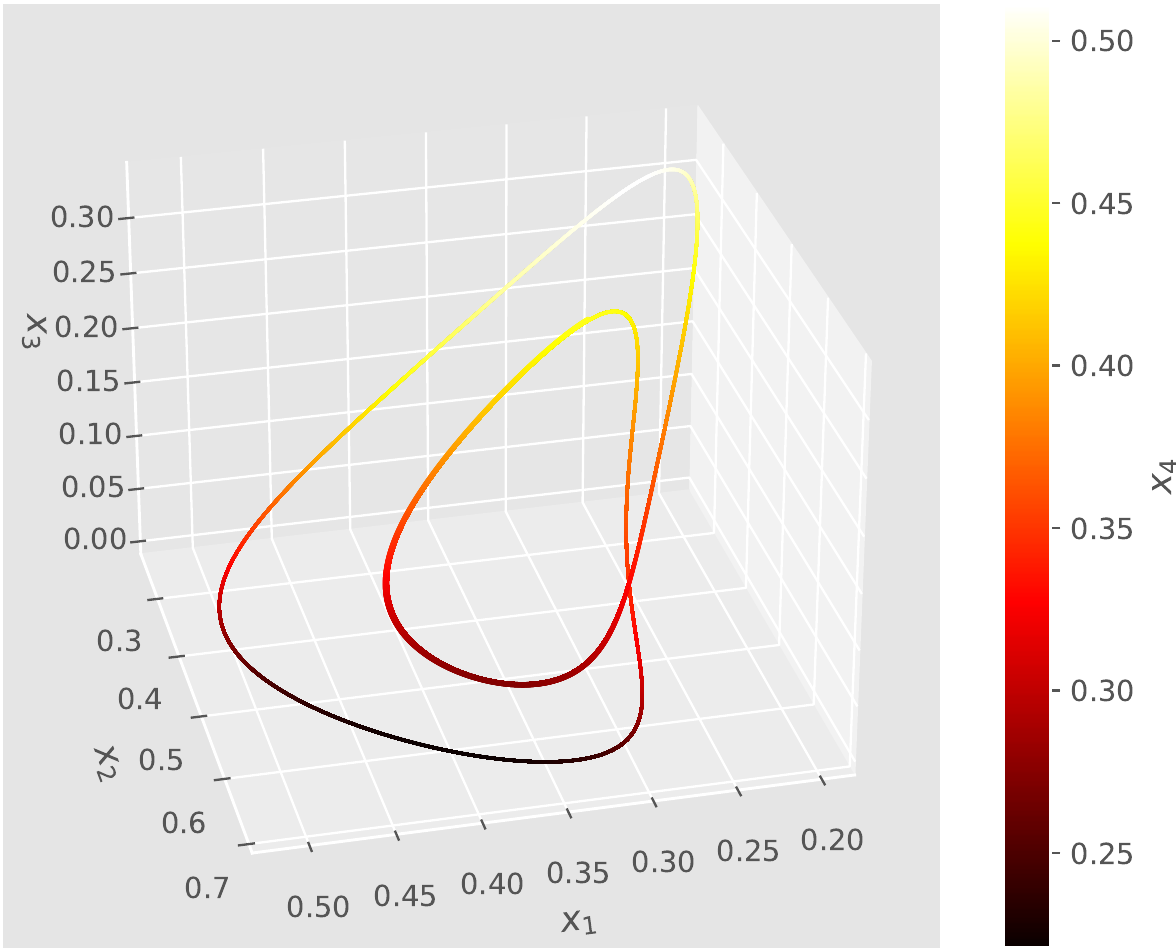
\includegraphics[width=\linewidth]{fig/lv4_cl4.png}
    \caption{cycle limite définit par XXX}
    \label{fig:cl4}
\end{figure}
\subsection{bifurcations}
\begin{equation}
R={\begin{bmatrix}1\\0.72\\1.53\\1.27\end{bmatrix}}\quad A =-{\begin{bmatrix}1&1.09s&1.52s&0\\0&0.72&0.3168s&0.9792s\\3.5649s&0&1.53&0.7191s\\1.5367s&0.6477s&0.4445s&1.27\end{bmatrix}}
\end{equation}
\begin{figure}[t!]
    \centering
    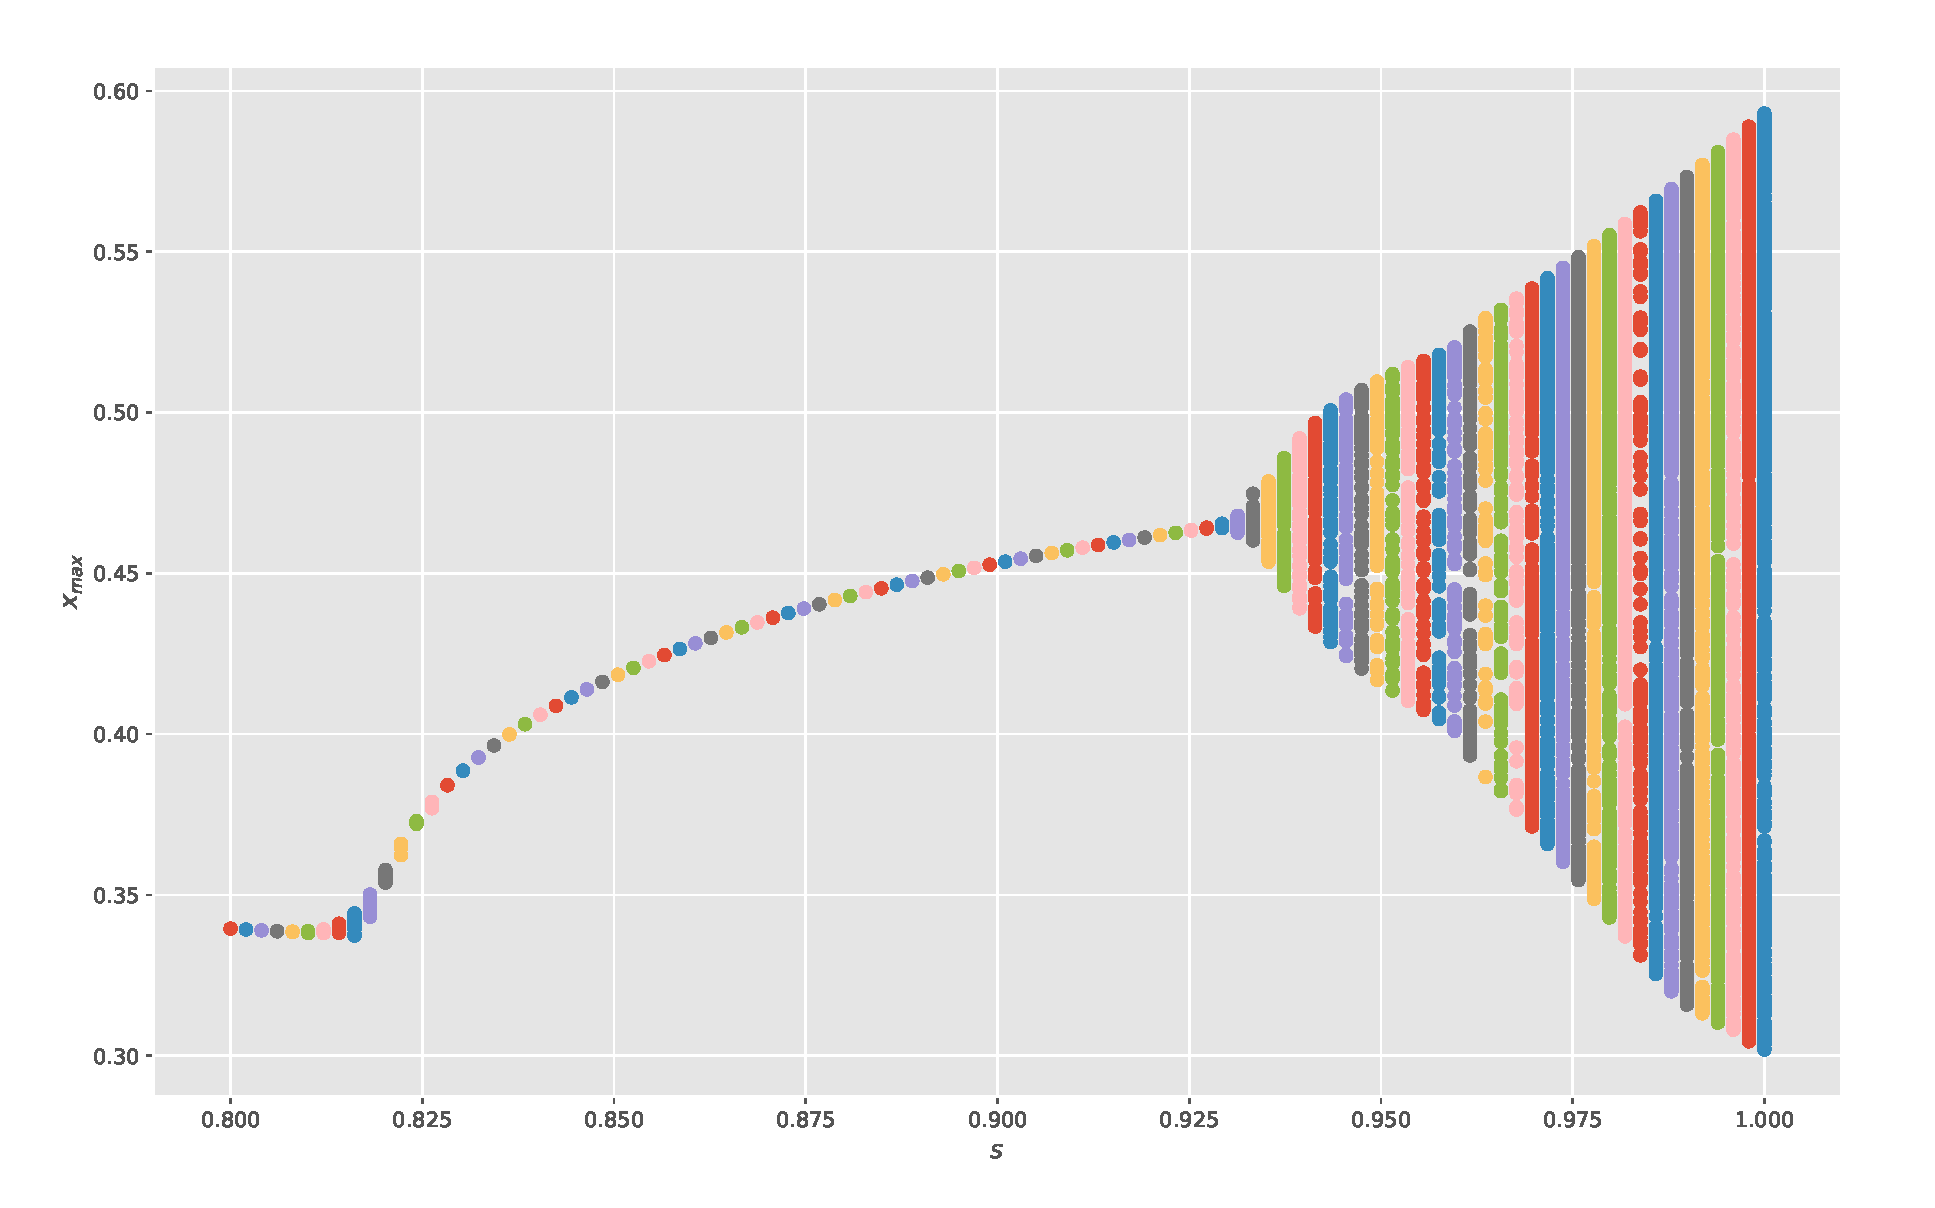
\includegraphics[width=\linewidth]{fig/lv4_bif.eps}
    \caption{test}
    \label{fig:bif4}
\end{figure}
\subsection{Cycle limite}
\begin{equation}
R={\begin{bmatrix}1\\0.72\\1.53\\1.27\end{bmatrix}}\quad A =-{\begin{bmatrix}1&1.0355&1.444&0\\0&0.72&0.30096&0.93024\\3.386655&0&1.53&0.683145\\1.459865&0.615315&0.422275&1.27\end{bmatrix}}
\end{equation}
\begin{figure}[t!]
    \centering
    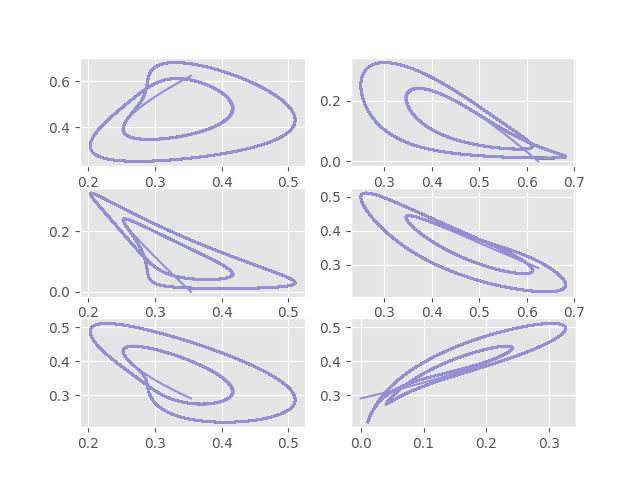
\includegraphics[width=\linewidth]{fig/lv4_cl.png}
    \caption{test}
    \label{fig:example}
\end{figure}
\subsection{Exposant de Liapounov}
\subsection{Bassin d'attraction}
\section{Conclusion}

\section{Annexes}
\section{bibliographie}
\nocite{*}
\printbibliography



%
%\appendices


\end{document}
